\textbf{Цель работы:} \\\indent
1) измерение объемов форвакуумной и высоковакуумной частей установки;\\\indent 
2) определение скорости откачки системы в стационарном режиме, а также 
по ухудшению и по улучшению вакуума. \\\indent
\textbf{Оборудование:} вакуумная установка с манометрами: масляным, 
термопарным и ионизационным. \\ 
\section*{Экспериментальная установка}

Установка состоит из форвакуумного баллона (ФБ), высоковакуумного диффузионного
насоса (ВН), высоковакуумного баллона (ВБ), масляного (М) и ионизационного (И) манометров,
термопарных манометров ($M_1$ и $M_2$), форвакуумного насоса (ФН) и кранов 
($K_1, \dots, K_6$).

\begin{figure}[h!]
    \centering
    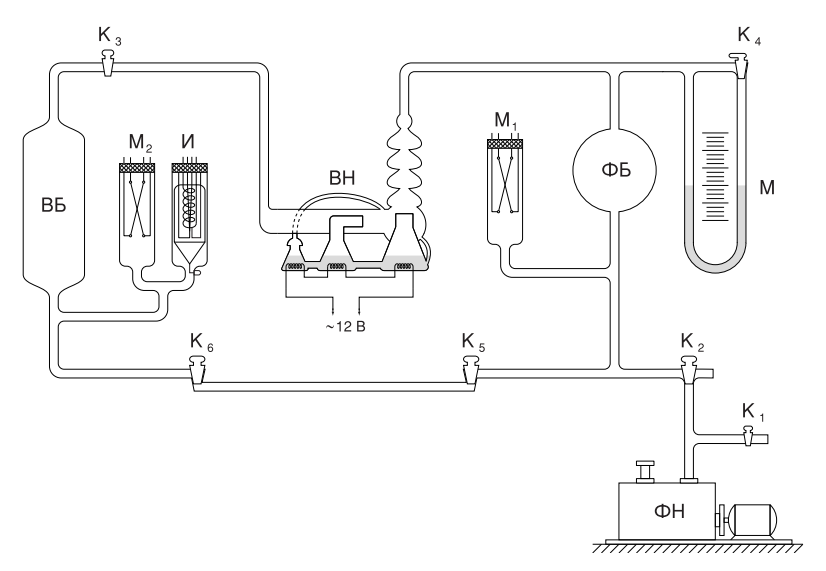
\includegraphics[height=8cm]{setup.png}
    \caption{Схема экспериментальной установки}
\end{figure}

\newpage

\section*{Теоретические сведения}
\subsection*{Откачка}
Пусть $W$ - объем газа, удаляемого из сосуда при данном давлении за 
единицу времени; $Q_{\text{д}}$ - кол-во газа, деосбирующегося с поверхности 
откачиваемого объема в ед.вр.; $Q_{\text{и}}$ - количество газа, принятое
извне; $Q_{\text{н}}$ - поток газа, поступающего из насоса назад в
откачиваемую систему. 
\begin{align}
    d(VP) &= (Q_{\text{д}} + Q_{\text{и}} + Q_{\text{н}}) dt \label{eq:dif}\\
    -VdP &= (PW - Q_{\text{д}} - Q_{\text{и}} - Q_{\text{н}}) dt
\end{align}
При достижении предельного вакуума $P_{\text{пр}}$:
\begin{align}
    \frac{dP}{dt} &= 0\\ 
    P_{\text{пр}}W = Q_{\text{д}} + Q_{\text{и}} + Q_{\text{н}} \Rightarrow W &= \frac{\sum Q_{\text{i}}}{P_{\text{пр}}}
\end{align}
Из \ref{eq:dif} и считая $Q_{\text{д}}, Q_{\text{и}}, Q_{\text{н}}$
постоянными, получаем:
\begin{equation}
P - P_{\text{пр}} = (P_0 - P_{\text{пр}})\exp{\left (-\frac{W}{V}t\right )}
\end{equation}
где $P_0$ - начальное давление ($P_0 \gg P_{\text{пр}}$) $\Rightarrow$
\begin{equation}
    P = P_0\exp(-\frac{W}{V}t)
\end{equation}

\subsection*{Течение газа через трубку}
Характер течения газа определяется размерами системы и длиной свободного 
пробега молекул. При понижении давления до форвакуумного длина свободного 
пробега меньше диаметра трубы, поэтому течение определяется вязкостью воздуха. 
При высоком вакууме роль длины свободного пробега молукл принимет диаметр
трубки. \\\indent 
Для количества газа, протекающего через трубку при высоком вакууме:
\begin{equation}
    \frac{d(PV)}{dt} = \frac{4}{3}r^3 \sqrt{\frac{2\pi RT}{\mu}} \frac{P_2 - P_1}{L}\label{eq:six_eq}
\end{equation}
Тогда пропускная способность трубы ($P = P_2, P_1 \ll P_2$):
\begin{equation}
    C_{\text{тр}} = \left (\frac{dV}{dt} \right ) = \frac{4}{3}\frac{r^3}{L} \sqrt{\frac{2\pi RT}{\mu}}  
\end{equation}

\newpage

\subsection*{Экспериментальные данные}

Зная объем трубки между кранами $K_5$ и $K_6$, найдем объемы форвакуумной 
и высоковакуумной частей ($V_{\text{фв}}$ и $V_{\text{вв}}$): $PV = const$.
\begin{table}[h!]
    \centering
    \begin{tabular}{|c|c|c|c|}
        \hline
        $V_{56}$, см$^3$ & $V_{\text{фв}}$, см$^3$ & $V_{\text{вв}}$, см$^3$ & $V_{\text{all}}$, см$^3$\\\hline
        500 & 2151 & 1280 & 3431\\\hline
    \end{tabular}
    \caption{Объемы установки}
\end{table}

Теперь найдем скорость откачки по улучшению вакуума:
\begin{figure*}[h!]
    \begin{minipage}{0.5\textwidth}
        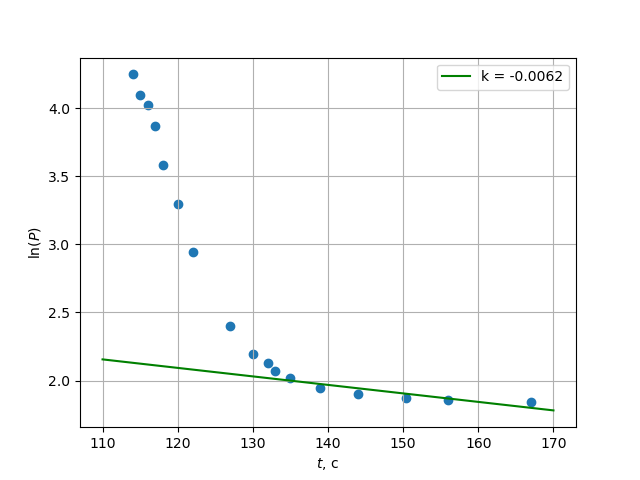
\includegraphics[width=10cm]{plotBetter1.png}
        \captionof{figure}{$\ln P (t); W = 463$ $\frac{\text{см}^3}{c}$}
    \end{minipage}
    \begin{minipage}{0.5\textwidth}
        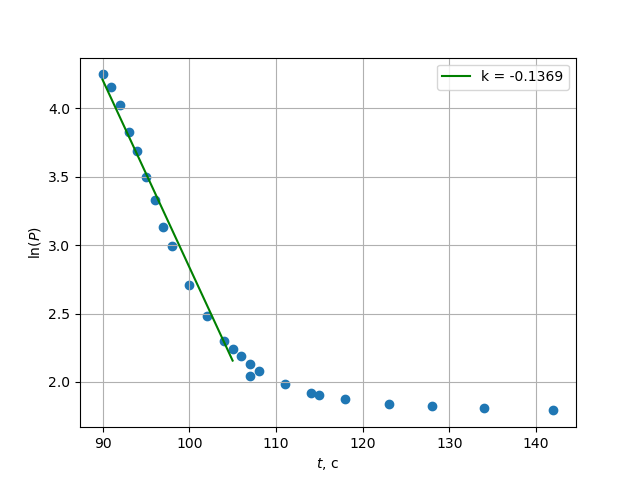
\includegraphics[width=10cm]{plotBetter2.png}
        \captionof{figure}{$\ln P (t); W = 470$ $\frac{\text{см}^3}{c}$}
    \end{minipage}

    \begin{minipage}{0.99\textwidth}
        \centering
        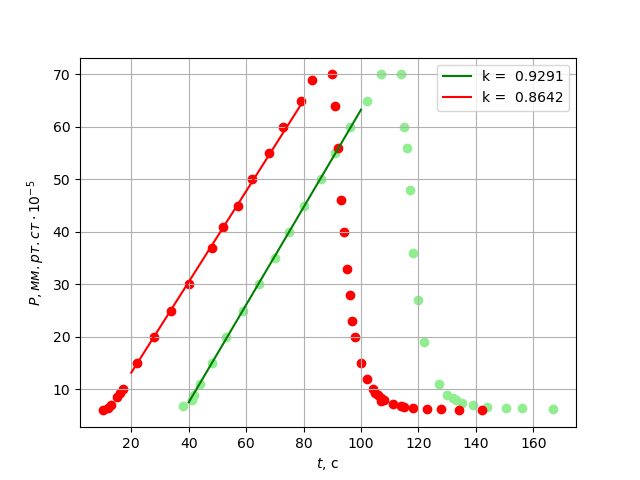
\includegraphics[width=11cm]{ALLPLOT.png}
        \captionof{figure}{График зависимости $P \text{ от } t$ при ухудшении
        и улучшении вакуума}
    \end{minipage}
\end{figure*}

Теперь оценим величину потока газа $Q_{\text{н}}$, поступающего из насоса
назад в откачиваемую систему:
\begin{align}
    V_{\text{вв}}dP = (Q_{\text{д}} + Q_{\text{и}})\\ 
    W P_{\text{пр}} = Q_{\text{д}} + Q_{\text{и}} + Q_{\text{н}}
\end{align}
Откуда $Q_{\text{н}} = 2.47$ $\frac{\text{см}^3 \cdot \text{Па}}{c}$.\\ 
После открывания крана $K_6$ мы ввели искуственную течь. Вакуум ухудшится. 
Установившееся давление $P_{\text{уст}} = 1.3\cdot 10^{-4}$ мм.рт.ст.\\ 
Давление со стороны форвакуумной части в свою очередь $P_{\text{фв}} = 3.8\cdot 10^{-3}$ мм.рт.ст.\\
Теперь рассчитаем производительность насоса по формуле:
\begin{align}
    P_{\text{уст}} W = P_{\text{пр}} W + \frac{d(PV)}{dt}
\end{align}
Последнее слагаемое вычисляется по $\ref{eq:six_eq}$ Откуда:
\begin{equation}
    W = \frac{d(PV)}{dt} \cdot \frac{1}{P_{\text{уст}} - P_{\text{пр}}} = 33 \text{ см}^3 / \text{с} 
\end{equation}



